\documentclass{report}
\usepackage[utf8]{inputenc}
\usepackage{amsmath, amsfonts, amsthm, graphicx, lipsum,enumerate}
\usepackage{hyperref}

\hypersetup{
    colorlinks=true,
    linkcolor=blue,
    urlcolor=red,
    pdftitle={Examen parcial},
    }
\usepackage[margin = 1 in]{geometry}
\usepackage{fancyvrb}
\usepackage{fancyhdr, lastpage}
\pagestyle{fancy}
\lhead{Examen parcial de Optimización de flujo en redes}
\rhead{Universidad Autónoma de Nuevo León}
\cfoot{Page \thepage\ of \pageref{LastPage}}

\usepackage{etoolbox} %Use carefully!
\patchcmd{\chapter}{\thispagestyle{plain}}{\thispagestyle{fancy}}{}{}

\usepackage[Glenn]{fncychap}
%Options: Sonny, Lenny, Glenn, Conny, Rejne, Bjarne, Bjornstrup


\usepackage{xcolor}
\usepackage{tikz}
\usepackage[most]{tcolorbox}

\newtcbtheorem{theo}%
  {Theorem}{}{theorem}
  
\usepackage{siunitx}
\usepackage{setspace}
\onehalfspacing
\begin{document}
\begin{center}
  { \LARGE Lic. Arnoldo Del Toro Peña}
\end{center}

\begin{enumerate}
  \item Professor May B. Wright suggest the following method for solving the shortest path problem with arbitrary arc lengths. Let $c_{min}$ = min $\{c ij : (i,j) \in A\}$. If $c_{min} <0$ add $|c_{min} |$ to the length of each arc
  in the network so that they all become nonnegative. Then use Dijkstra’s algorithm to solve the
  shortest path problem. Professor Wright claims that the optimal solution of the transformed
  problem is also an optimal solution of the original problem. Prove or disprove her claim.

  Esto es válido para grafos que no contienen ciclos negativos como el siguiente:
  \begin{figure}[h!t]
    \centering
    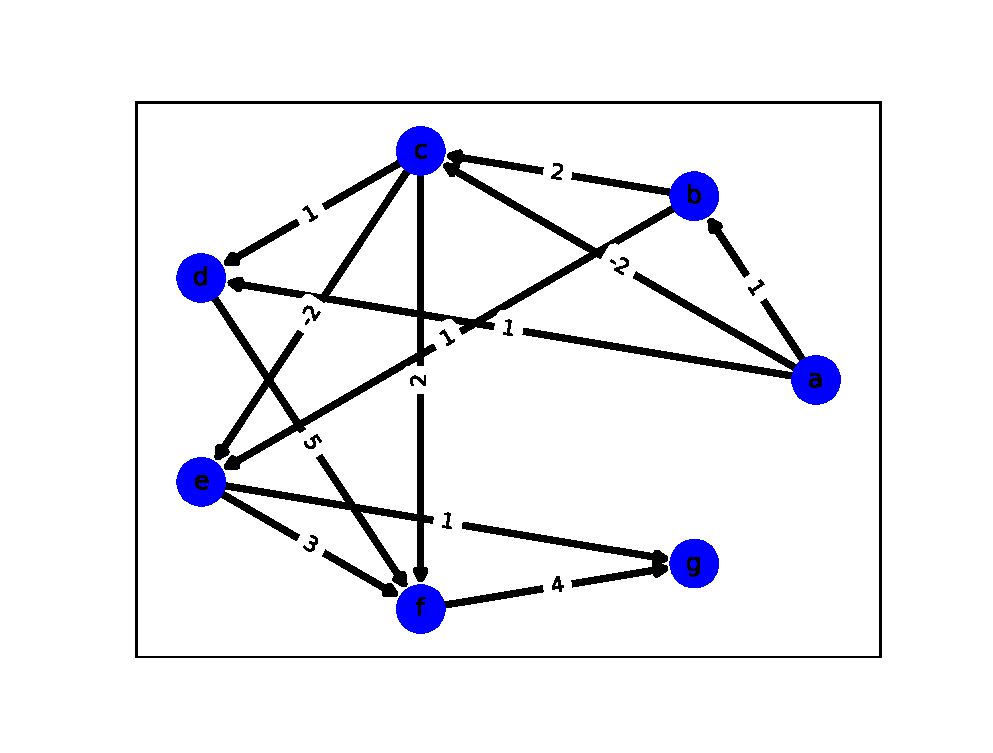
\includegraphics[scale = 0.4]{ejemplo6.eps}
    \caption{Grafo sin ciclo negativo}
    \label{sinciclonegativo}
  \end{figure} 

  En este problema la distancia más corta: -3 y la ruta más corta es:  [a, c, e, g], ahora si aplicamos el método propuesto por el profesor May, obtenemos el siguiente grafo:
  \begin{figure}[h!t]
    \centering
    \includegraphics[scale = 0.4]{ejemplo10.eps}
    \caption{Grafo sin ciclo negativo}
    \label{sinciclonegativo2}
  \end{figure}

  En este problema la distancia más corta: 3 y la ruta más corta es:  [a, c, e, g]

  Pero no funciona con un grafo que contiene un ciclo negativo, veamos el siguiente grafo:
  \begin{figure}[h!t]
    \centering
    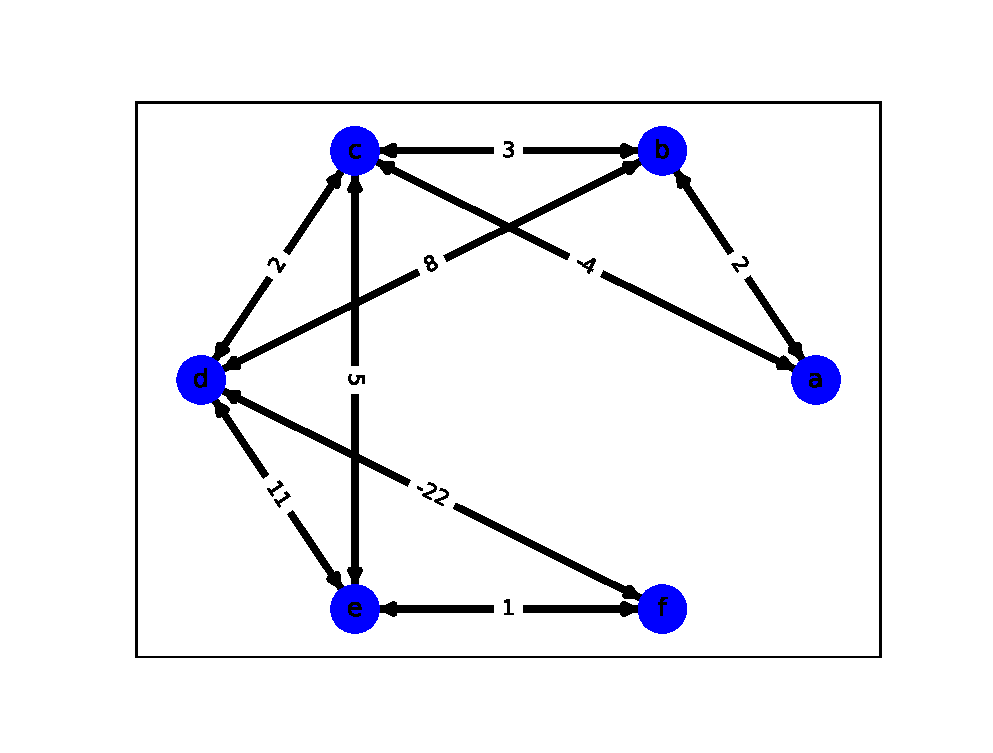
\includegraphics[scale = 0.4]{ejemplo11.eps}
    \caption{Grafo con ciclo negativo}
    \label{conciclonegativo}
  \end{figure}
  \newpage
  En este problema, como ya habíamos visto en clase, si el grafo contiene un ciclo negativo entonces no podemos obtener una solución óptima de todos los nodos existentes, por lo cuál este grafo no tiene una ruta más corta, sin embargo al aplicar el método del profesor eliminamos el ciclo negativo por lo cuál podremos encontrar una solución al problema, esto es contradictorio al problema original. Veamos el grafo al aplicar la suma de 22 a cada uno de los arcos:
  \begin{figure}[h!t]
    \centering
    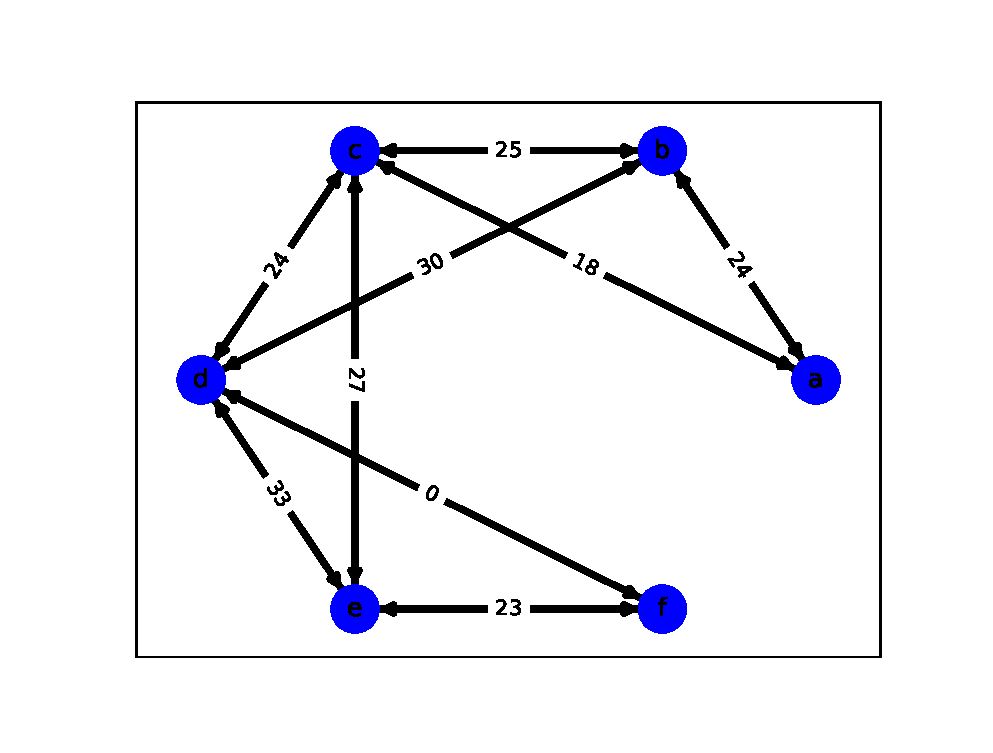
\includegraphics[scale = 0.4]{ejemplo12.eps}
    \caption{Grafo con ciclo negativo}
    \label{conciclonegativo2}
  \end{figure}

  En este caso tenemos la ruta más corta con un valor de 54 y la ruta: [a,b,d,f] lo cual no coincide con el problema original, debido a que como ya se mencionó el problema original contiene un ciclo negativo lo cual podemos estar pasando varias veces por el mismo camino generando cada vez una solución más negativa entonces el método del profesor (como se mencionó al principio) solo funciona en grafos sin ciclos negativos, por lo cual la afirmación de que ambas soluciones óptimas son iguales, es falsa.

  \item Describe an algorithm for updating the shortest path distances from node s to every other node if we add a new node (n+1) and some arcs incident to this node. Consider the following three cases: 1) all arc lenghts are nonnegative and node (n+1) has only incoming arcs; 2) all arc lenghts are nonnegative and node (n+1) has incoming as well as outgoing arcs; and 3) arc lenghts are arbitrary, but node (n+1) has only incoming arcs.
  
  Se asume que todos los nodos a excepción del nodo n+1 tienen etiqueta obtenida mediante el algoritmo Bellman-Ford.
    \begin{enumerate}[1)]
      \item Como todo costo nuevo al nodo (n+1) es $\geq 0$, y solo hay arcos de entrada entonces podemos hacer lo siguiente para todo nodo i que se conecte con el nodo n+1:
      \begin{center}
        Etiqueta[n+1] = $\infty$ \\ 
        mientras etiqueta[n+1]  $> c_{i,n+1} + $ etiqueta[i] \\
        hacer etiqueta[n+1] = $c_{i,n+1} + $ etiqueta[i] \\
        etiqueta[n+1][predecesor] = i
      \end{center}      

      \item Repetiremos el inciso 1:
      \begin{center}
        Etiqueta[n+1] = $\infty$ \\ 
        mientras etiqueta[n+1]  $> c_{i,n+1} + $ etiqueta[i] \\
        hacer etiqueta[n+1] = $c_{i,n+1} + $ etiqueta[i] \\
        etiqueta[n+1][predecesor] = i
      \end{center}

      Pero agregaremos estos pasos extra que haremos para todo nodo j que sea la llegada desde el nodo n+1:
      \begin{center}
        mientras etiqueta[j]  $> c_{n+1,j} + $ etiqueta[n+1] \\
        hacer etiqueta[j] = $c_{n+1,j} + $ etiqueta[n+1] \\
        etiqueta[j][predecesor] = n+1
      \end{center}

      \item En este caso repetiremos el inciso 1:
      \begin{center}
        Etiqueta[n+1] = $\infty$ \\ 
        mientras etiqueta[n+1]  $> c_{i,n+1} + $ etiqueta[i] \\
        hacer etiqueta[n+1] = $c_{i,n+1} + $ etiqueta[i] \\
        etiqueta[n+1][predecesor] = i
      \end{center}

      Pero al igual que el inciso 2 tenemos que agregar unas líneas extras debido a que en este caso las longitudes de los arcos son arbitrarias por lo cual puede existir un ciclo negativo.

      \begin{center}
        Hacer la ruta al nodo n+1 \\
        si ruta es un ciclo negativo \\
        entonces imprimir ciclo negativo
      \end{center}

    \end{enumerate}

    \item If we use Floyd-Warshall algorithm, how could we identify that the graph contains a negative cycle? Explain your answer.
    
    En el algoritmo de Floyd-Warshall podemos terminar todo el algoritmo y al final revisar en la matriz resultante si en las posiciones de nodos identidad es decir $(i,i)$ existe un valor menor a 0 (o durante el proceso), entonces esto quiere decir que nuestro grafo tiene un ciclo negativo, esto pasa por la forma en que se inicializan estas posiciones, si recordamos en los lugares de identidad les asignamos el valor de 0 ya que no tiene un costo ir del nodo i al nodo i, pero si nuestro algoritmo encuentra que hay una ``mejora" para ir del nodo i al nodo i es por que entonces existe un ciclo de i a i y al tener el valor negativo nos da como resultado la definición de ciclo negativo.






\end{enumerate}
\end{document}